\documentclass{article}

\usepackage{fancyhdr}
\usepackage{extramarks}
\usepackage{amsmath}
\usepackage{amsthm}
\usepackage{amsfonts}
\usepackage{tikz}
\usepackage[plain]{algorithm}
\usepackage{algpseudocode}
\usepackage{enumerate}
\usepackage{tikz,forest}
\usepackage{multicol}
\usepackage{enumitem}
\usepackage{adjustbox}
%\usepackage[demo]{graphicx}

%
% Basic Document Settings
%

\topmargin=-0.45in
\evensidemargin=0in
\oddsidemargin=0in
\textwidth=6.5in
\textheight=9.0in
\headsep=0.25in

\linespread{1.1}

\pagestyle{fancy}
\lhead{\hmwkAuthorName}
\chead{\hmwkClass : \hmwkTitle}
\rhead{\firstxmark}
\lfoot{\lastxmark}
\cfoot{\thepage}

\renewcommand\headrulewidth{0.4pt}
\renewcommand\footrulewidth{0.4pt}

\setlength\parindent{0pt}

%
% Create Problem Sections
%

\newcommand{\enterProblemHeader}[1]{
\nobreak\extramarks{}{Problem \arabic{#1} continued on next page\ldots}\nobreak{}
\nobreak\extramarks{Problem \arabic{#1} (continued)}{Problem \arabic{#1} continued on next page\ldots}\nobreak{}
}

\newcommand{\exitProblemHeader}[1]{
\nobreak\extramarks{Problem \arabic{#1} (continued)}{Problem \arabic{#1} continued on next page\ldots}\nobreak{}
\stepcounter{#1}
\nobreak\extramarks{Problem \arabic{#1}}{}\nobreak{}
}

\setcounter{secnumdepth}{0}
\newcounter{partCounter}
\newcounter{homeworkProblemCounter}
\setcounter{homeworkProblemCounter}{1}
\nobreak\extramarks{Problem \arabic{homeworkProblemCounter}}{}\nobreak{}

%
% Homework Problem Environment
%
% This environment takes an optional argument. When given, it will adjust the
% problem counter. This is useful for when the problems given for your
% assignment aren't sequential. See the last 3 problems of this template for an
% example.
%
\newenvironment{homeworkProblem}[1][-1]{
\ifnum#1>0
\setcounter{homeworkProblemCounter}{#1}
\fi
\section{Problem \arabic{homeworkProblemCounter}}
\setcounter{partCounter}{1}
\enterProblemHeader{homeworkProblemCounter}
}{
\exitProblemHeader{homeworkProblemCounter}
}

%
% Homework Details
%   - Title
%   - Due date
%   - Class
%   - Section/Time
%   - Instructor
%   - Author
%

\newcommand{\hmwkTitle}{Problem Set\ \#4}
\newcommand{\hmwkDueDate}{October 15, 2017}
\newcommand{\hmwkClass}{CIS 520}
%\newcommand{\hmwkClassTime}{Section A}
\newcommand{\hmwkClassInstructor}{Lyle Ungar, Shivani Agarwal}
\newcommand{\hmwkAuthorName}{Eric Oh}

%
% Title Page
%

\title{
\vspace{2in}
\textmd{\textbf{\hmwkClass:\ \hmwkTitle}}\\
\normalsize\vspace{0.1in}\small{Due\ on\ \hmwkDueDate\ }\\
\vspace{0.1in}\large{\textit{\hmwkClassInstructor}}
\vspace{3in}
}

\author{\textbf{\hmwkAuthorName}}
\date{}

\renewcommand{\part}[1]{\textbf{\large Part \Alph{partCounter}}\stepcounter{partCounter}\\}

%
% Various Helper Commands
%

% Useful for algorithms
\newcommand{\alg}[1]{\textsc{\bfseries \footnotesize #1}}

% For derivatives
\newcommand{\deriv}[1]{\frac{\mathrm{d}}{\mathrm{d}x} (#1)}

% For partial derivatives
\newcommand{\pderiv}[2]{\frac{\partial}{\partial #1} (#2)}

% Integral dx
\newcommand{\dx}{\mathrm{d}x}

% Alias for the Solution section header
\newcommand{\solution}{\textbf{\large Solution}}

% Probability commands: Expectation, Variance, Covariance, Bias
\newcommand{\E}{\mathrm{E}}
\newcommand{\Var}{\mathrm{Var}}
\newcommand{\Cov}{\mathrm{Cov}}
\newcommand{\Bias}{\mathrm{Bias}}

\begin{document}

\maketitle
\begin{center}
{\normalsize \noindent Collaborators: Jiarui Lu} \\
\end{center}
\pagebreak

\begin{homeworkProblem}

Convolutional Neural Network

\solution

\begin{enumerate}

\item Each neuron in the first hidden layer would require $48150$ weights for a fully connected neural network. 
\item Using a filter of size $21 \times 14 \times 3$ results in $882$ weights for a single neuron. 
\item The size of the output image from the Conv layer is 
\begin{equation*} \frac{W-F+2P}{S}+1\end{equation*}
where $W$ is the input volume size, $F$ is the size of the Conv layer filter, $P$ is the amount of zero padding on the border, and $S$ is the stride size. Thus, for a $105 \times 154$ input image, a $21 \times 14$ filter, 0 padding, and a stride of 7, the output image is $13 \times 21$, resulting in $273$ neurons. 
\item The first output of the $3 \times 3 \times 2$ output is given by applying the $3 \times 3 \times 1$ filter 1 to the input image with a stride of 1. The second is found by applying the $3 \times 3 \times 1$ filter 2 to the input image with a stride of 1. This results in an output of
\[ \left( \begin{array}{ccc}
0 & -2 & 0 \\
-2 & -4 & -2 \\
0 & -2 & 0
\end{array} \right)
%
\left( \begin{array}{ccc}
0 & 3 & 0 \\
3 & 6 & 3 \\
0 & 3 & 0
\end{array} \right)
\]
\end{enumerate}
\end{homeworkProblem}

\begin{homeworkProblem}

Convex Sets

\solution

\begin{enumerate}

\item 
\begin{enumerate}[label=(\alph*)]
\item Yes, this is a convex set because it is a Euclidean norm ball in $\mathbb{R}^3$ centered at the origin with radius $\sqrt{8}$. 
\item No, this is not a convex set. Take the points $(0,0,3)$ and $(0,0,-3)$ both in C. The line segment connecting the two points contains the origin, which is not in C. 
\item No, this is not a convex set. Take the points $(0,4,0)$ and $(0,0,4)$ both in C. The line segment connecting the two points contains $(0,2,2)$, which is not in C. 
\item Yes, this is a convex set. Note that each of the constraints can be written as the intersection of two halfspaces. For example, $0 \leq x_1 \leq 1$ is equivalent to the intersection of $a_1^Tx+b_1 \leq 0$ and $a_2^Tx+b_2 \leq 0$ where $a_1=(-1,0,0), b_1=0, a_2=(1,0,0), b_2=-1$. Thus, C is the intersection of halfspaces and is thus a convex set. 
\item Yes, this is a convex set as it is the intersection of $l_{\infty}$ and $l_1$ norm balls.
\end{enumerate}

\item 
\begin{enumerate}[label=(\alph*)]
\item f is both convex and concave due to it being an affine function.
\item f is not a convex function. To see this, note that we can write f as $f(x)=x^TAx$ where
A = \[ \left( \begin{array}{ccc}
1 & 0 & 0 \\
0 & 1 & 0 \\
0 & 0 & -1
\end{array} \right)
\]
f would be a convex function if A is positive semi-definite. Since A is a diagonal matrix, the eigenvalues are given by the diagonal entires and thus we check if either A or -A has all non-negative eigenvalues. We note that since neither A nor -A has all non-negatives eigenvalues, A is not positive semi-definite and thus f is not convex. 
\item f is a convex set. To see this, note that we can write f as $f(x)=x^TAx$ where
A = \[ \left( \begin{array}{ccc}
-1 & 0 & 0 \\
0 & 0 & 0 \\
0 & 0 & -1
\end{array} \right)
\]
f would be a convex function if A is positive semi-definite. Since A is a diagonal matrix, the eigenvalues are given by the diagonal entires and thus we check if either A or -A has all non-negative eigenvalues. We note that since -A has all non-negative eigenvalues, A is positive semi-definite and thus f is convex.
\item f is convex because it is the supremum of convex functions. 
\item f is convex because it is the $L_1$ norm of x. 
\end{enumerate}
\end{enumerate}
\end{homeworkProblem}

\begin{homeworkProblem}

Optimization and Duality

\solution

\begin{enumerate}
\item $L(x_1,x_2,\lambda) = 4x_1 + 3x_2 + \lambda(x_1^2+x_2^2-1)$
\item The minimum values of $x_1$ and $x_2$ are given by
\begin{align*}
\frac{dL}{dx_1} &= 4 + 2\lambda x_1 \equiv 0 \hspace{0.2in} \Rightarrow \hspace{0.2in} \hat{x}_1=-\frac{2}{\lambda} \\
\frac{dL}{dx_2} &= 3 + 2\lambda x_2 \equiv 0 \hspace{0.2in} \Rightarrow \hspace{0.2in} \hat{x}_2=-\frac{3}{2\lambda} \\
\end{align*}
Note that the second derivatives are positive, indicating that they are indeed minima. The dual function is then given by
\begin{align*}
\phi(\lambda) = \text{inf}_x L(x_1,x_2,\lambda) = 4\left(-\frac{2}{\lambda}\right) + 3\left(-\frac{3}{2\lambda}\right) + \lambda\left(\frac{4}{\lambda^2}\right)+\lambda\left(\frac{9}{4\lambda^2}\right)-\lambda = -\frac{4}{\lambda} - \frac{9}{4\lambda}-\lambda
\end{align*}
\item To solve the dual problem, we initially attempt to find an unconstrained maximum of the dual objective. If this maximum is greater than 0, than we have a solution to the constrained dual problem. 
\begin{align*}
\frac{d\phi(\lambda)}{d\lambda} = \frac{4}{\lambda^2} + \frac{9}{4\lambda^2} - 1 \equiv 0 \hspace{0.2in} \Rightarrow \hspace{0.2in} \hat{\lambda} = \pm \frac{5}{2}
\end{align*}
Since $\hat{\lambda} = \frac{5}{2}$ is greater than 0, we have a solution to the constrained dual problem. Thus, a solution to the primal problem is given by $\hat{x}_1 =  -\frac{2}{2.5} = -0.8$ and $\hat{x}_2 = -\frac{3}{5} = -0.6$. This solution does not lie in the Euclidean ball of the primal constraint because $(-0.8)^2 + (-0.6)^2 = 1$, rather it lies on it. 
\end{enumerate}
\end{homeworkProblem}

\begin{homeworkProblem}

Kernel Functions

\solution

\begin{enumerate}
\item Let $\phi(x) = \sqrt{c}\phi_1(x)$. Then
\begin{align*}
\phi(x)^T\phi(x') = \sqrt{c}\phi_1^T(x) \sqrt{c}\phi(x') = c\phi_1^T(x)\phi_1^T(x') = cK_1(x,x') = K(x,x')
\end{align*}

\item Let $\phi(x) = (\phi_1(x),\phi_2(x))$. Then
\begin{align*}
\phi(x)^T\phi(x') &= (\phi_1(x),\phi_2(x))^T (\phi_1(x'),\phi_2(x'))\\
&= \phi_1^T(x)\phi_1(x') + \phi_2^T(x)\phi_2(x') \\
&= K_1(x,x')+K_2(x,x') = K(x,x')
\end{align*}

\item A mapping $\phi$ cannot exist because dot products always sum elements. If either $\phi_1(x)$ or $\phi_2(x)$ were made to be negative, the dot product would then result in a summation. 
\item Let $\phi(x)=\phi_1(f(x))$. Then
\begin{align*}
\phi(x)^T\phi(x') = \phi_1^T(f(x))\phi_1(f(x')) = K_1(f(x),f(x')) = K(x,x')
\end{align*}
\end{enumerate}
\end{homeworkProblem}

\begin{homeworkProblem}

SVM and Kernels

\solution

\begin{enumerate}

\item 

\begin{itemize}
\item For $q=1$, the training decision boundary is shown in the plot below.
\begin{center}
\begin{minipage}[t]{\linewidth}
%\raggedright
\centering
\adjustbox{valign=t}{%
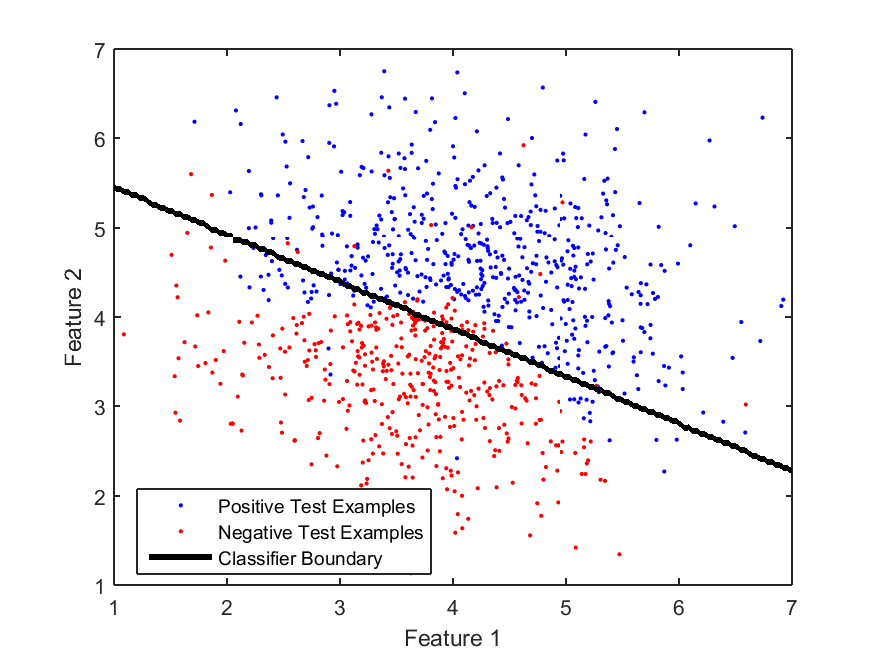
\includegraphics[width=\linewidth]{hw4_release/SVM-problem/Plots/SVM_polynomial_train_degree_1.png}%
}
\medskip
\end{minipage}
\end{center}

The testing decision boundary is shown below. 
\begin{center}
\begin{minipage}[t]{\linewidth}
%\raggedright
\centering
\adjustbox{valign=t}{%
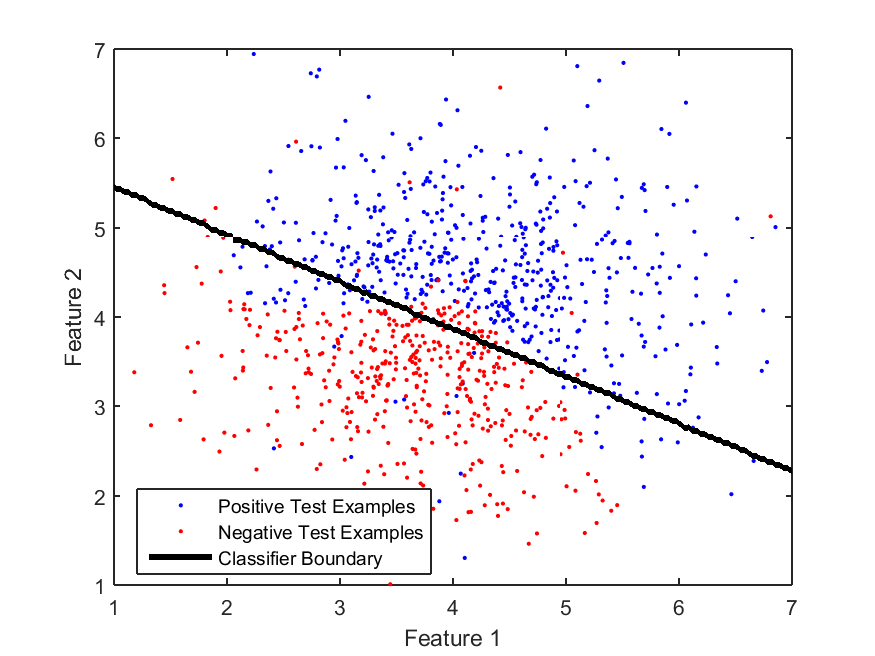
\includegraphics[width=\linewidth]{hw4_release/SVM-problem/Plots/SVM_polynomial_test_degree_1.png}%
}
\medskip
\end{minipage}
\end{center}

\item For $q=2$, the training decision boundary is shown in the plot below.
\begin{center}
\begin{minipage}[t]{\linewidth}
%\raggedright
\centering
\adjustbox{valign=t}{%
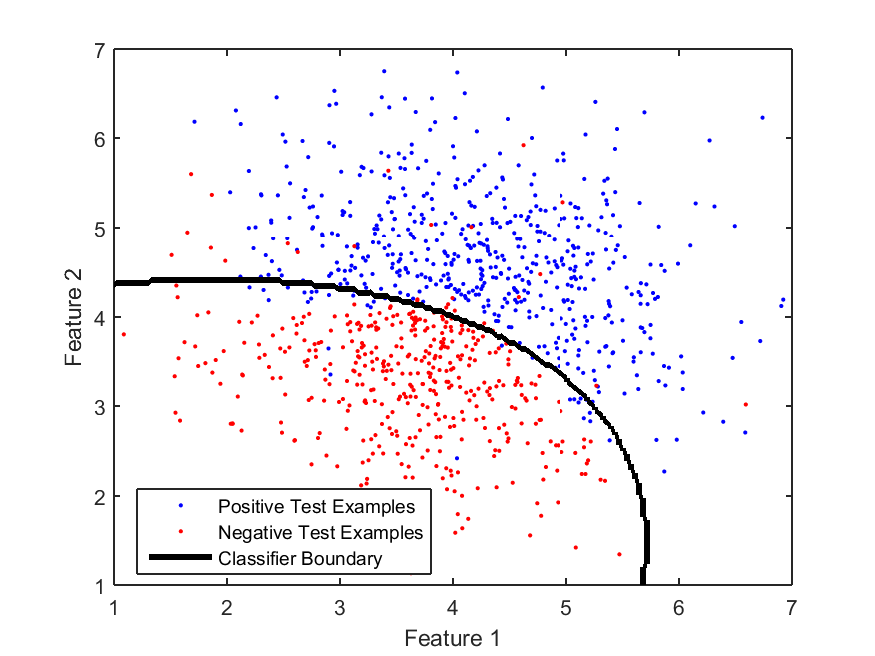
\includegraphics[width=\linewidth]{hw4_release/SVM-problem/Plots/SVM_polynomial_train_degree_2.png}%
}
\medskip
\end{minipage}
\end{center}

The testing decision boundary is shown below. 
\begin{center}
\begin{minipage}[t]{\linewidth}
%\raggedright
\centering
\adjustbox{valign=t}{%
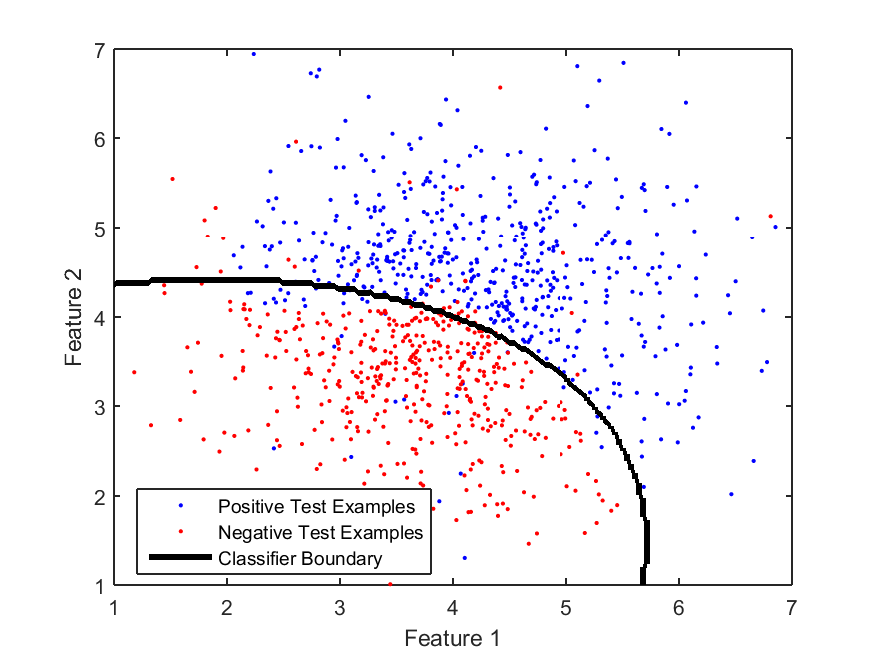
\includegraphics[width=\linewidth]{hw4_release/SVM-problem/Plots/SVM_polynomial_test_degree_2.png}%
}
\medskip
\end{minipage}
\end{center}

\item For $q=3$, the training decision boundary is shown in the plot below.
\begin{center}
\begin{minipage}[t]{\linewidth}
%\raggedright
\centering
\adjustbox{valign=t}{%
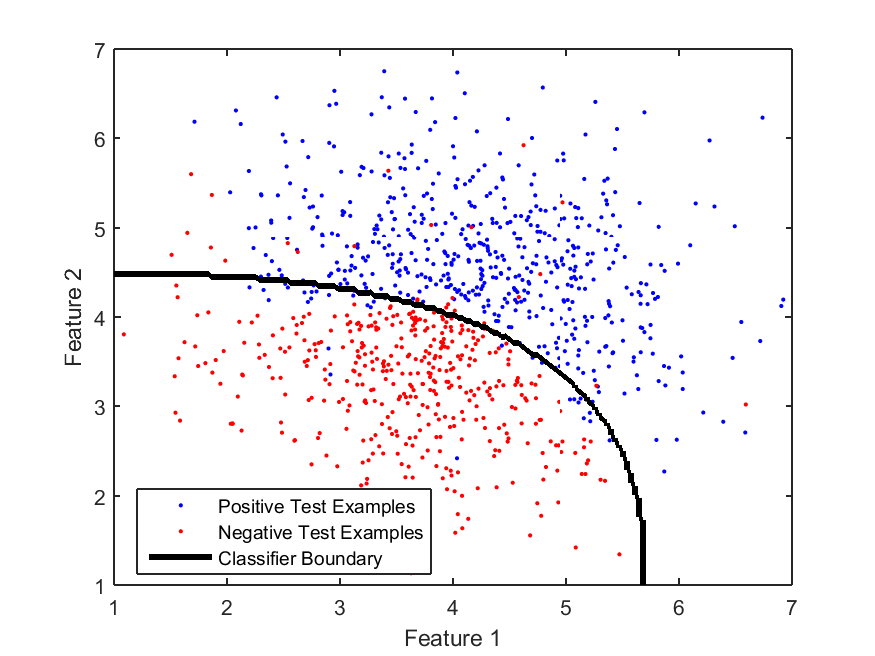
\includegraphics[width=\linewidth]{hw4_release/SVM-problem/Plots/SVM_polynomial_train_degree_3.png}%
}
\medskip
\end{minipage}
\end{center}

The testing decision boundary is shown below. 
\begin{center}
\begin{minipage}[t]{\linewidth}
%\raggedright
\centering
\adjustbox{valign=t}{%
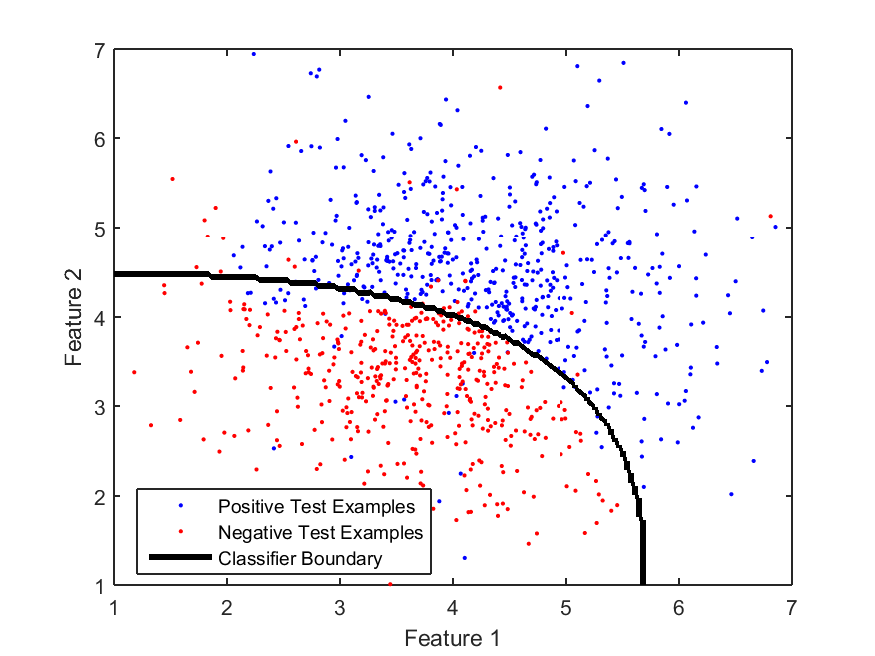
\includegraphics[width=\linewidth]{hw4_release/SVM-problem/Plots/SVM_polynomial_test_degree_3.png}%
}
\medskip
\end{minipage}
\end{center}

\item For $q=4$, the training decision boundary is shown in the plot below.
\begin{center}
\begin{minipage}[t]{\linewidth}
%\raggedright
\centering
\adjustbox{valign=t}{%
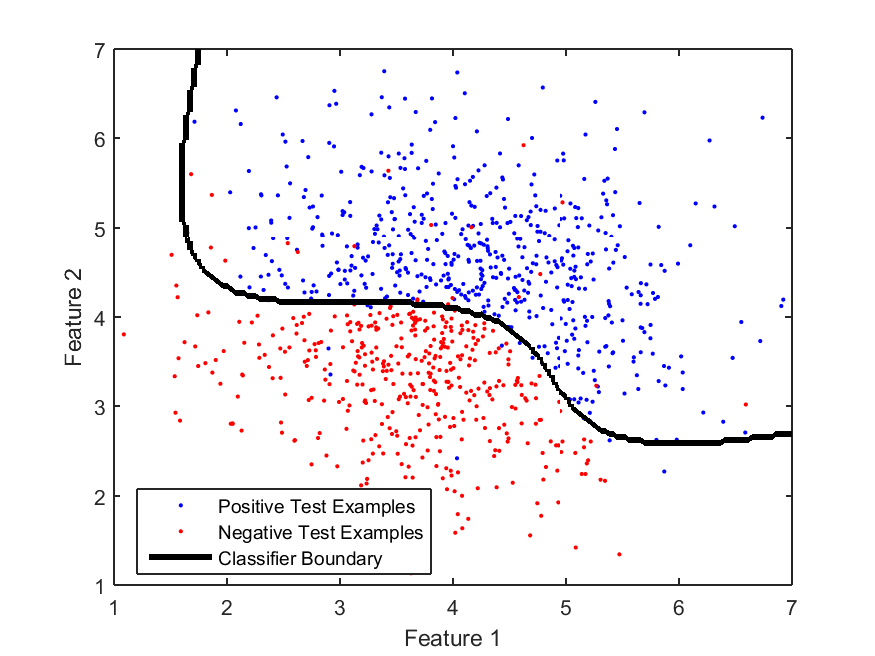
\includegraphics[width=\linewidth]{hw4_release/SVM-problem/Plots/SVM_polynomial_train_degree_4.png}%
}
\medskip
\end{minipage}
\end{center}

The testing decision boundary is shown below. 
\begin{center}
\begin{minipage}[t]{\linewidth}
%\raggedright
\centering
\adjustbox{valign=t}{%
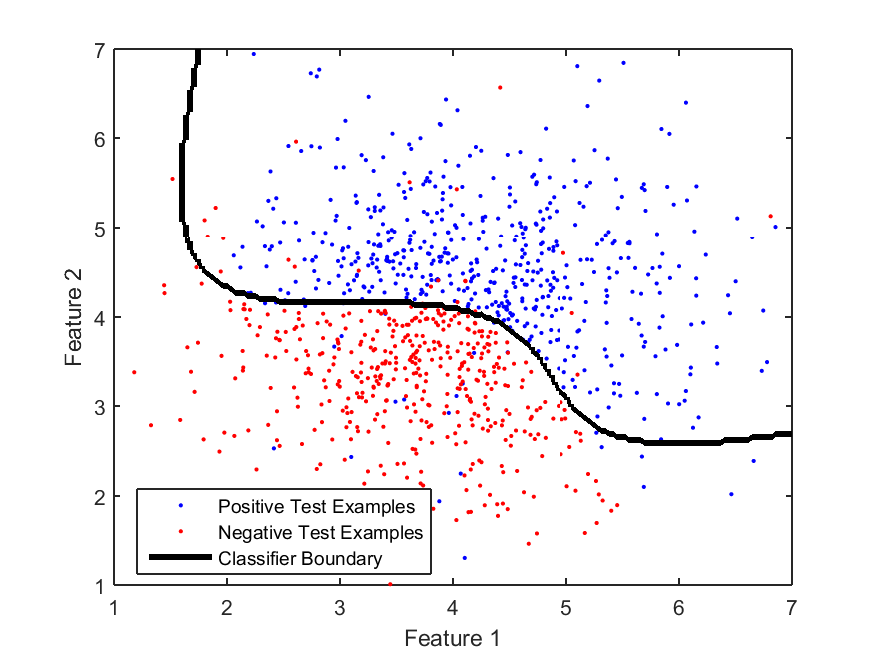
\includegraphics[width=\linewidth]{hw4_release/SVM-problem/Plots/SVM_polynomial_test_degree_4.png}%
}
\medskip
\end{minipage}
\end{center}

\item For $q=5$, the training decision boundary is shown in the plot below.
\begin{center}
\begin{minipage}[t]{\linewidth}
%\raggedright
\centering
\adjustbox{valign=t}{%
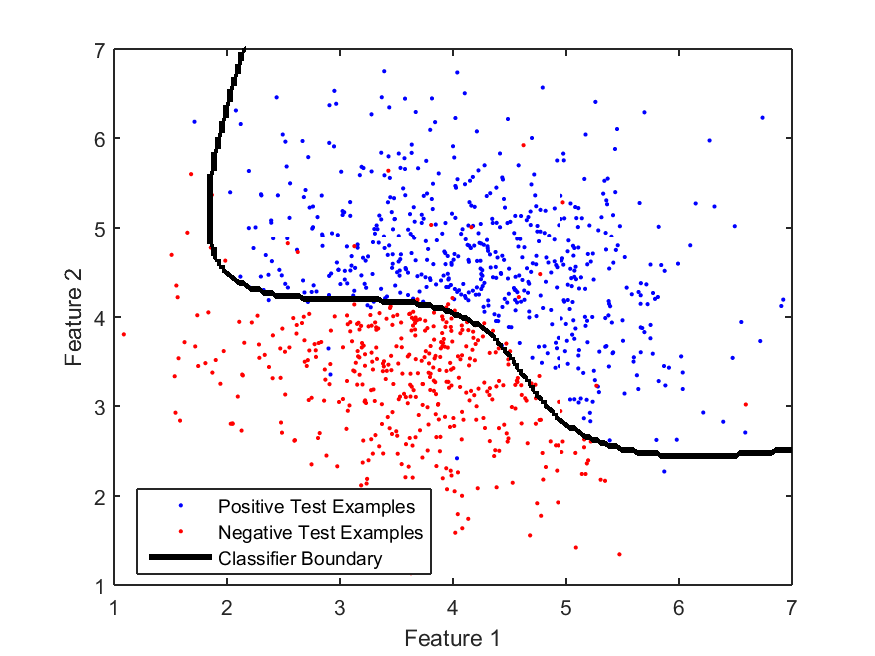
\includegraphics[width=\linewidth]{hw4_release/SVM-problem/Plots/SVM_polynomial_train_degree_5.png}%
}
\medskip
\end{minipage}
\end{center}

The testing decision boundary is shown below. 
\begin{center}
\begin{minipage}[t]{\linewidth}
%\raggedright
\centering
\adjustbox{valign=t}{%
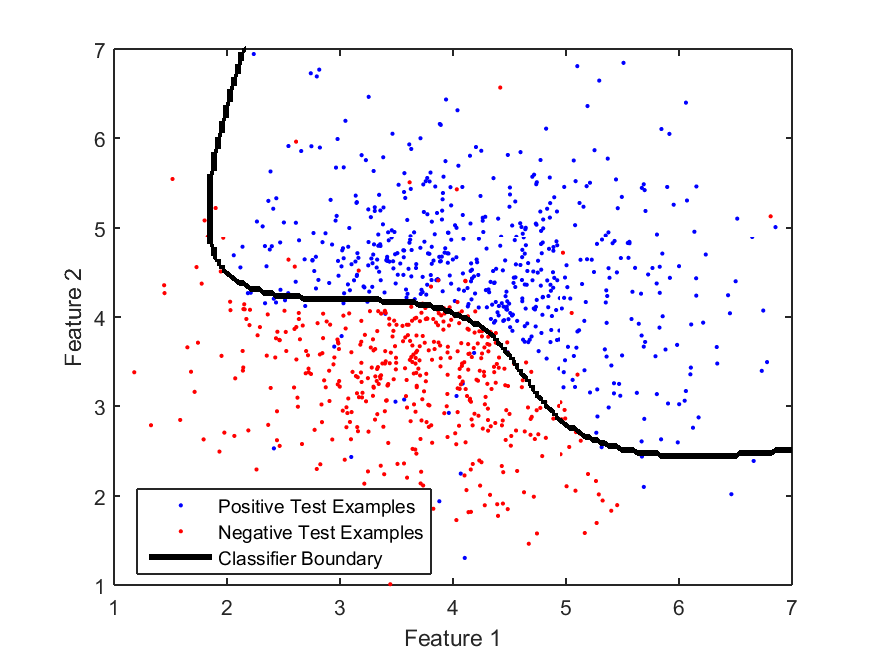
\includegraphics[width=\linewidth]{hw4_release/SVM-problem/Plots/SVM_polynomial_test_degree_5.png}%
}
\medskip
\end{minipage}
\end{center}

\item The training and testing error achieved by each value of q is shown in the plot below. The value of q that achieves the lowest test error is $q=4$. 
\begin{center}
\begin{minipage}[t]{\linewidth}
%\raggedright
\centering
\adjustbox{valign=t}{%
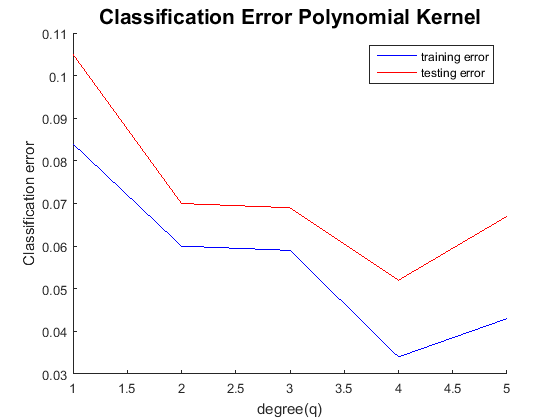
\includegraphics[width=\linewidth]{hw4_release/SVM-problem/Plots/ClassificationErr_degree.png}%
}
\medskip
\end{minipage}
\end{center}
\end{itemize}

\item 

\begin{itemize}
\item For $\sigma=0.01$, the training decision boundary is shown in the plot below.
\begin{center}
\begin{minipage}[t]{\linewidth}
%\raggedright
\centering
\adjustbox{valign=t}{%
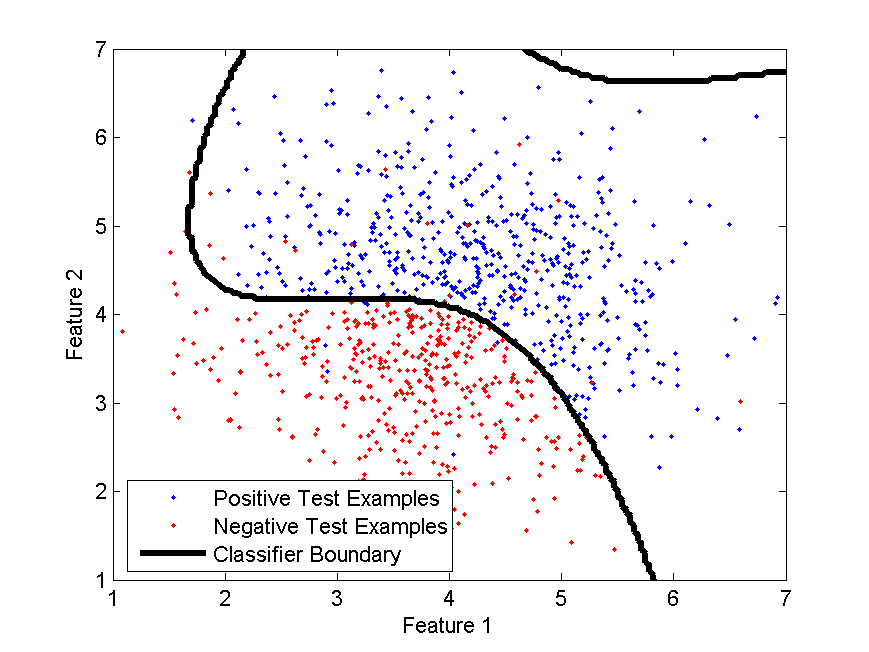
\includegraphics[width=\linewidth]{hw4_release/SVM-problem/Plots/SVM_RBF_train_sigma_001.png}%
}
\medskip
\end{minipage}
\end{center}

The testing decision boundary is shown below. 
\begin{center}
\begin{minipage}[t]{\linewidth}
%\raggedright
\centering
\adjustbox{valign=t}{%
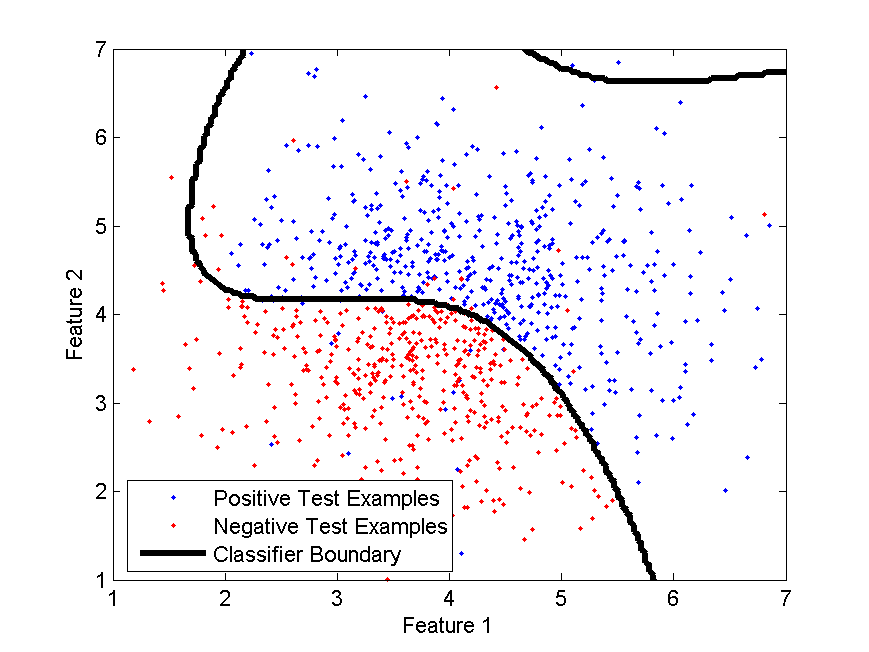
\includegraphics[width=\linewidth]{hw4_release/SVM-problem/Plots/SVM_RBF_test_sigma_001.png}%
}
\medskip
\end{minipage}
\end{center}

\item For $\sigma=1$, the training decision boundary is shown in the plot below.
\begin{center}
\begin{minipage}[t]{\linewidth}
%\raggedright
\centering
\adjustbox{valign=t}{%
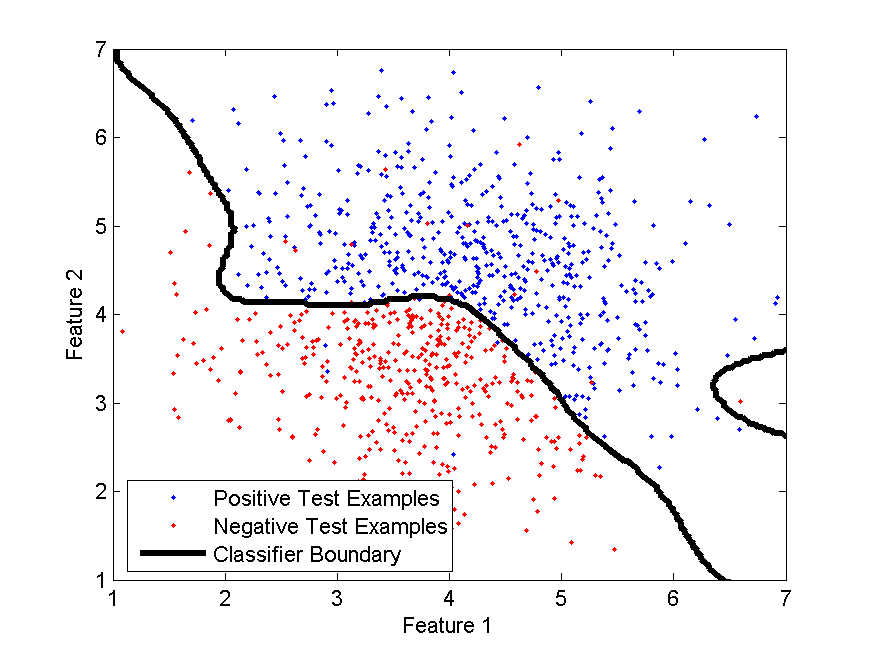
\includegraphics[width=\linewidth]{hw4_release/SVM-problem/Plots/SVM_RBF_train_sigma_1.png}%
}
\medskip
\end{minipage}
\end{center}

The testing decision boundary is shown below. 
\begin{center}
\begin{minipage}[t]{\linewidth}
%\raggedright
\centering
\adjustbox{valign=t}{%
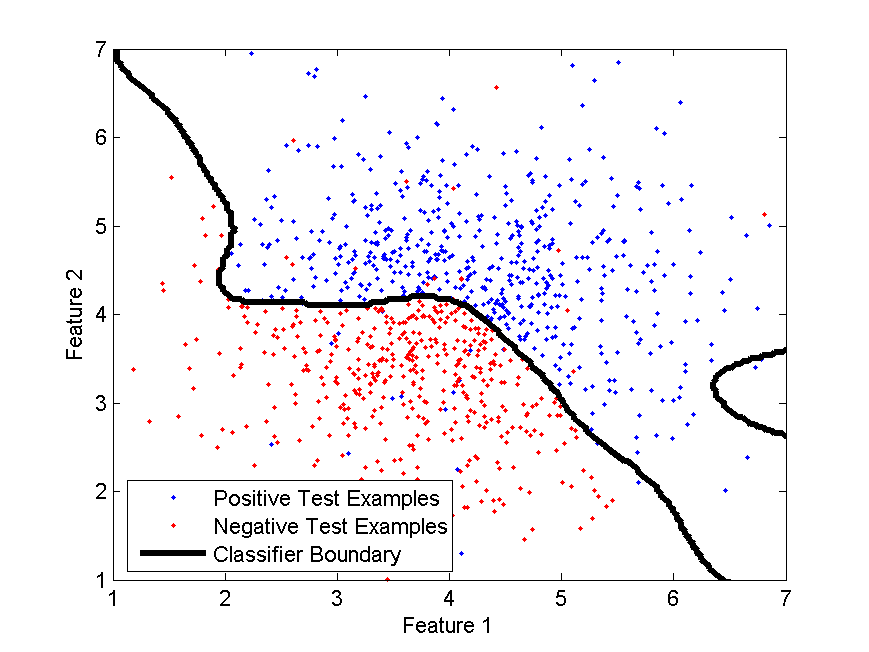
\includegraphics[width=\linewidth]{hw4_release/SVM-problem/Plots/SVM_RBF_test_sigma_1.png}%
}
\medskip
\end{minipage}
\end{center}

\item For $\sigma=10$, the training decision boundary is shown in the plot below.
\begin{center}
\begin{minipage}[t]{\linewidth}
%\raggedright
\centering
\adjustbox{valign=t}{%
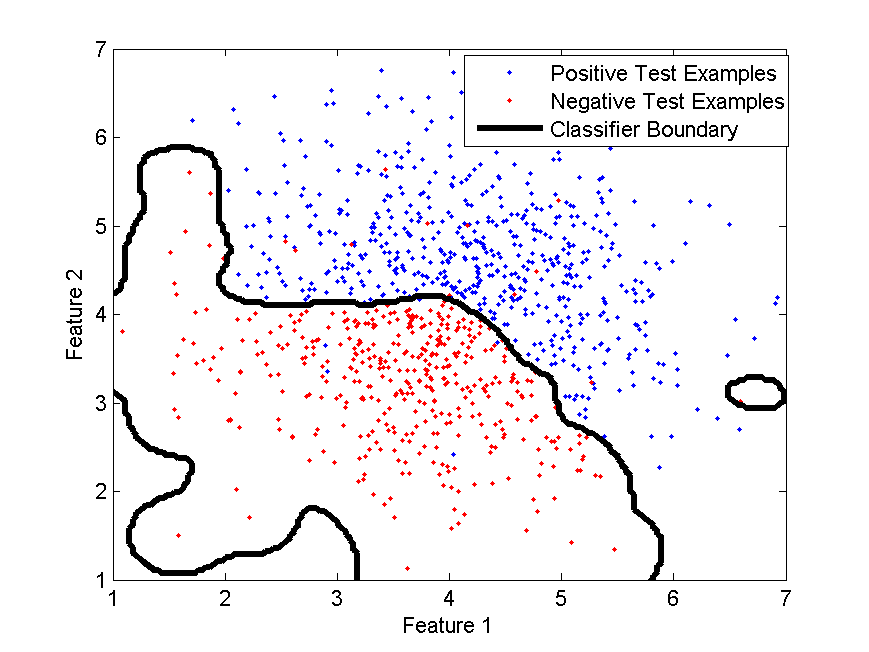
\includegraphics[width=\linewidth]{hw4_release/SVM-problem/Plots/SVM_RBF_train_sigma_10.png}%
}
\medskip
\end{minipage}
\end{center}

The testing decision boundary is shown below. 
\begin{center}
\begin{minipage}[t]{\linewidth}
%\raggedright
\centering
\adjustbox{valign=t}{%
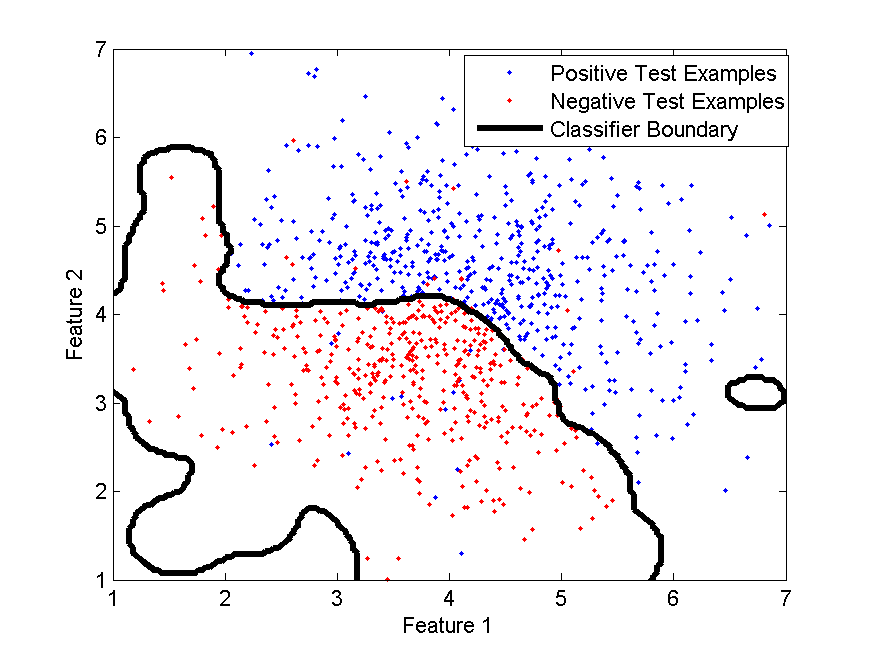
\includegraphics[width=\linewidth]{hw4_release/SVM-problem/Plots/SVM_RBF_test_sigma_10.png}%
}
\medskip
\end{minipage}
\end{center}

\item For $\sigma=100$, the training decision boundary is shown in the plot below.
\begin{center}
\begin{minipage}[t]{\linewidth}
%\raggedright
\centering
\adjustbox{valign=t}{%
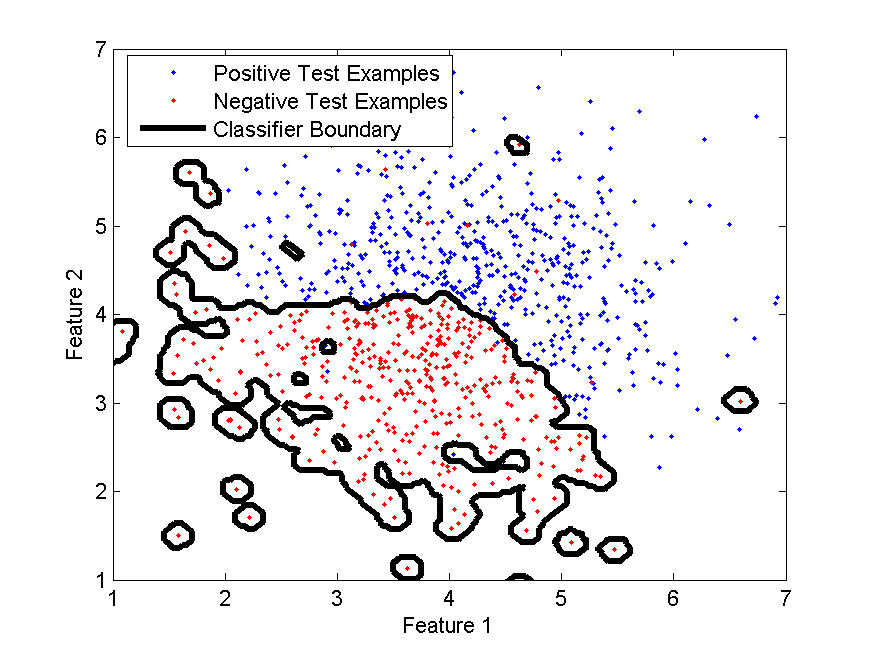
\includegraphics[width=\linewidth]{hw4_release/SVM-problem/Plots/SVM_RBF_train_sigma_100.png}%
}
\medskip
\end{minipage}
\end{center}

The testing decision boundary is shown below. 
\begin{center}
\begin{minipage}[t]{\linewidth}
%\raggedright
\centering
\adjustbox{valign=t}{%
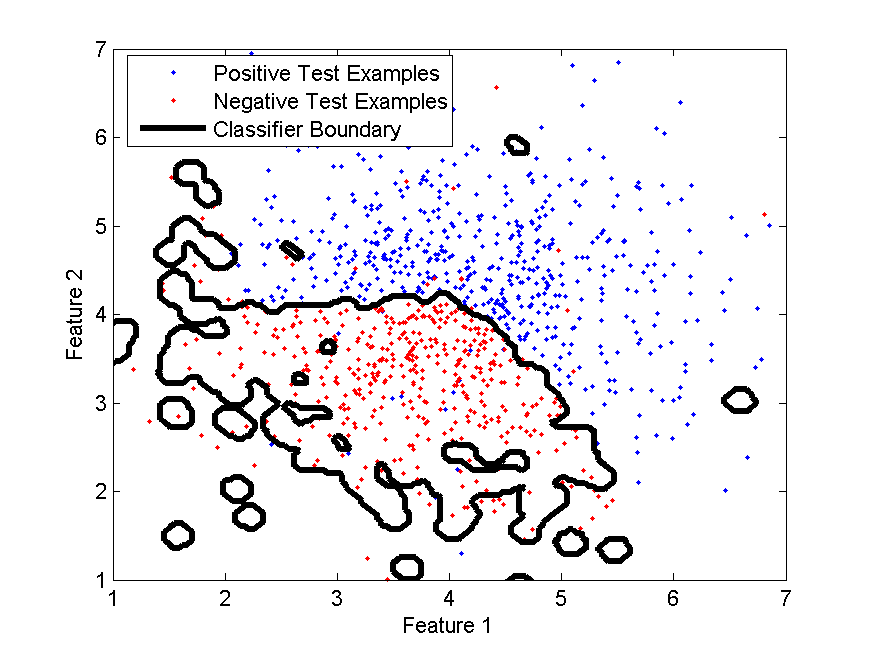
\includegraphics[width=\linewidth]{hw4_release/SVM-problem/Plots/SVM_RBF_test_sigma_100.png}%
}
\medskip
\end{minipage}
\end{center}

\item For $\sigma=1000$, the training decision boundary is shown in the plot below.
\begin{center}
\begin{minipage}[t]{\linewidth}
%\raggedright
\centering
\adjustbox{valign=t}{%
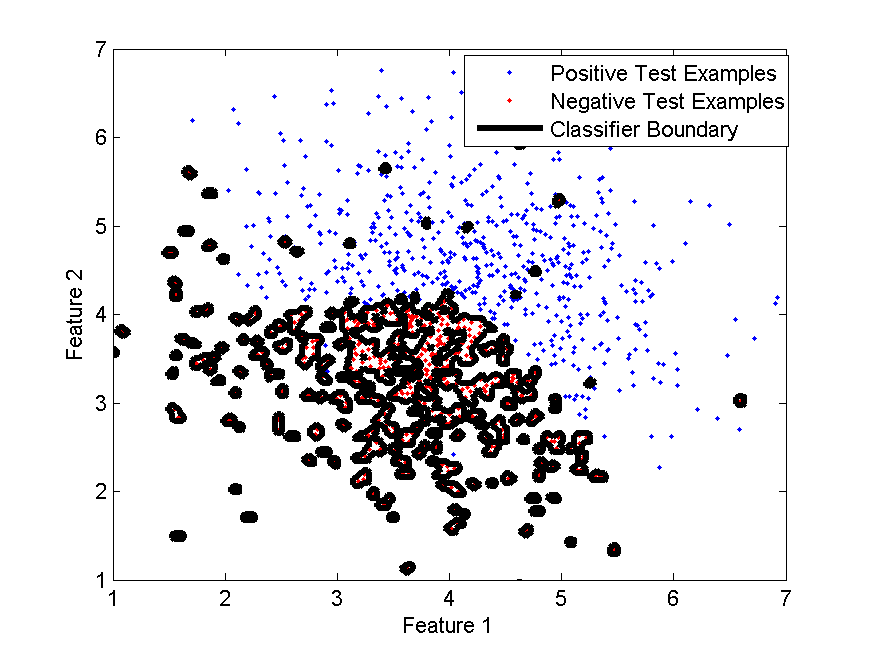
\includegraphics[width=\linewidth]{hw4_release/SVM-problem/Plots/SVM_RBF_train_sigma_1000.png}%
}
\medskip
\end{minipage}
\end{center}

The testing decision boundary is shown below. 
\begin{center}
\begin{minipage}[t]{\linewidth}
%\raggedright
\centering
\adjustbox{valign=t}{%
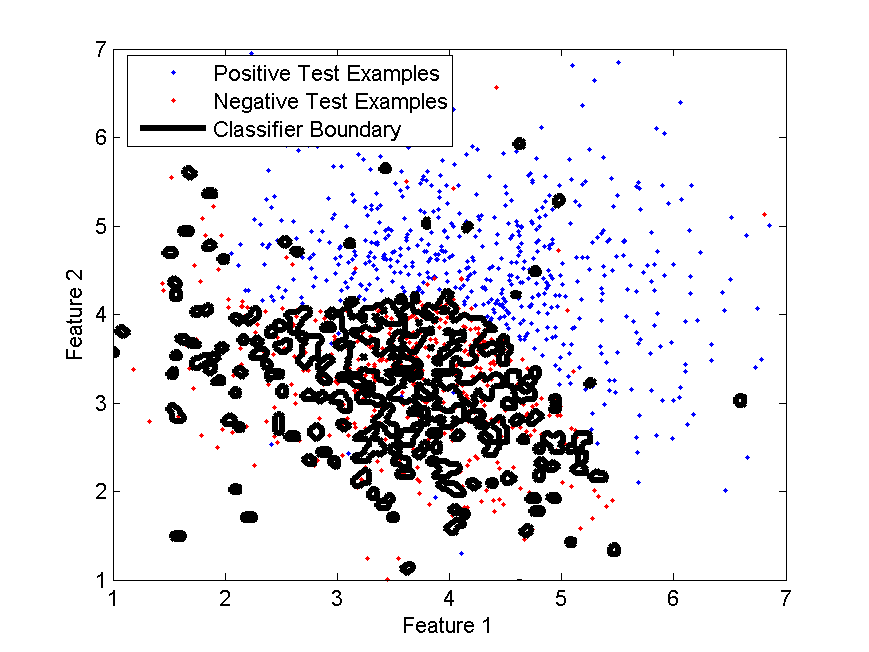
\includegraphics[width=\linewidth]{hw4_release/SVM-problem/Plots/SVM_RBF_test_sigma_1000.png}%
}
\medskip
\end{minipage}
\end{center}

\item The training and testing error achieved by each value of $\sigma$ is shown in the plot below. The value of $\sigma$ that achieves the lowest test error is $\sigma=1$ or $\sigma=10$ (equal). 
\begin{center}
\begin{minipage}[t]{\linewidth}
%\raggedright
\centering
\adjustbox{valign=t}{%
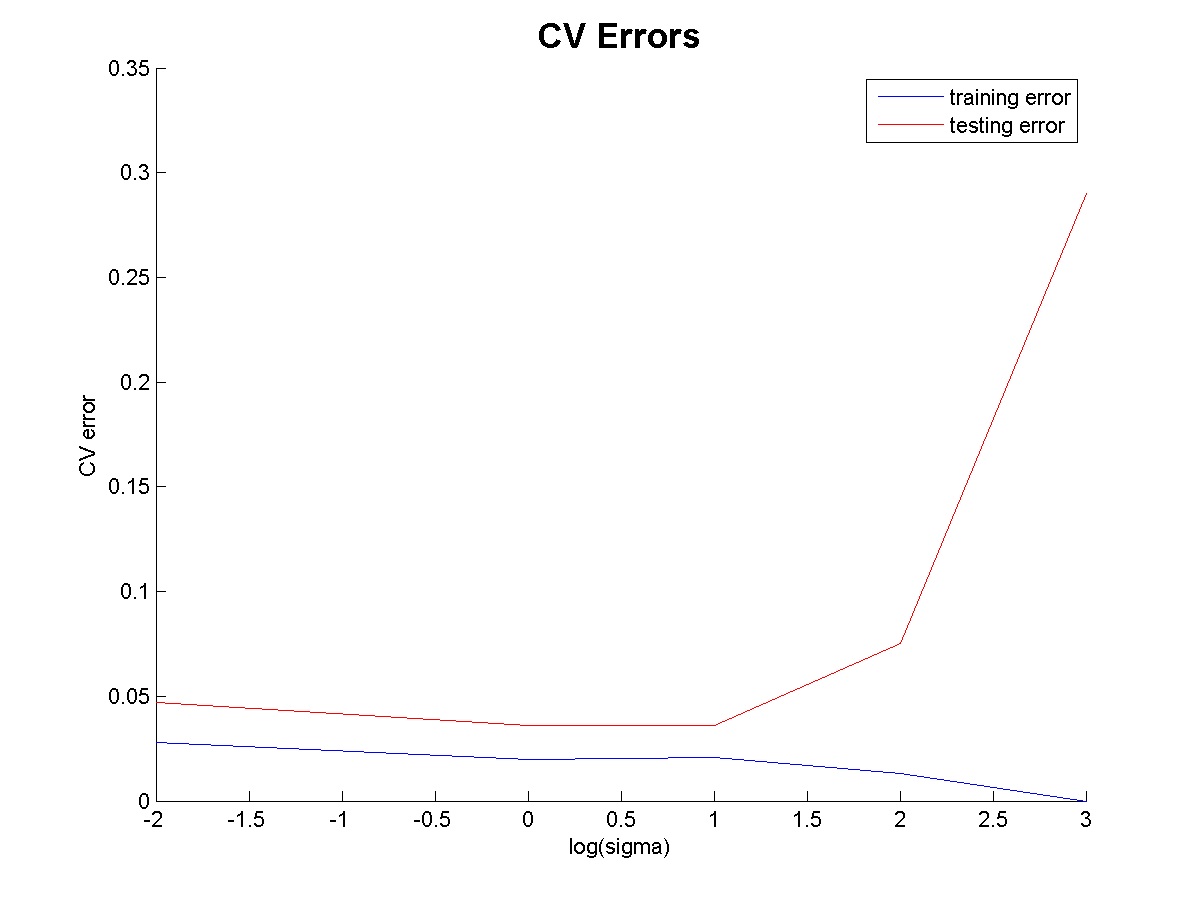
\includegraphics[width=\linewidth]{hw4_release/SVM-problem/Plots/CV.png}%
}
\medskip
\end{minipage}
\end{center}
\end{itemize}

\item 

\begin{itemize}

\item The following plot shows the training, testing, and cross-validation errors for the polynomial kernel. The CV error shows that $q=4$ is the best kernel parameter, which corresponds to the lowest test error found in part 1. 
\begin{center}
\begin{minipage}[t]{\linewidth}
%\raggedright
\centering
\adjustbox{valign=t}{%
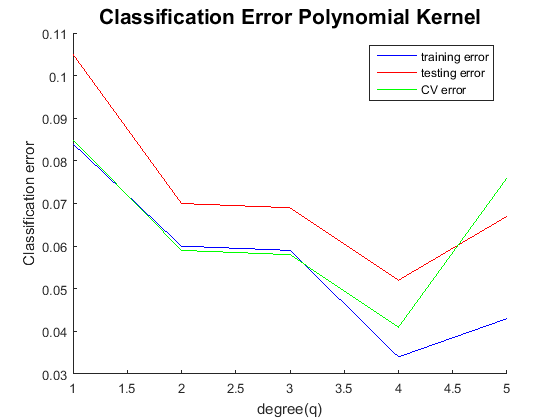
\includegraphics[width=\linewidth]{hw4_release/SVM-problem/Plots/ClassificationErr_degree_CV.png}%
}
\medskip
\end{minipage}
\end{center}

\item The following plot shows the training, testing, and cross-validation errors for the RBF kernel. The CV error shows that $\sigma=1$ is the best kernel parameter, which does correspond to the lowest test error found in part 2. This confirms that cross-validation is a great way to select the kernel parameters.   
\begin{center}
\begin{minipage}[t]{\linewidth}
%\raggedright
\centering
\adjustbox{valign=t}{%
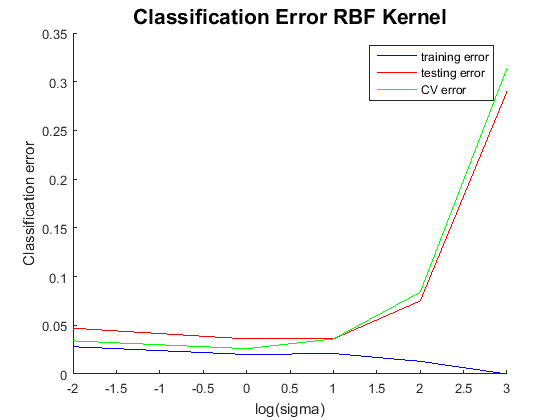
\includegraphics[width=\linewidth]{hw4_release/SVM-problem/Plots/ClassificationErr_Sigma_CV.png}%
}
\medskip
\end{minipage}
\end{center} 
\end{itemize}

\item The test accuracy for the polynomial kernel was 0.95181 and 0.96386 for the RBF kernel. 
\end{enumerate}
\end{homeworkProblem}

\end{document}